%the margins are different
%font size is differnt
%citations ka mark is left
%do u need letterpaper??
%list on page 2 isnt correct
%page 2 featurez left marginsd
%check references , check whr ur content is lying , check sapcing araound table and bw iamges
\documentclass[10pt]{article}
\usepackage{xcolor}
\usepackage[parfill]{parskip}
\usepackage{ragged2e}

\usepackage{fancyhdr}
\usepackage[a4paper]{geometry}
\usepackage{enumitem} % for controlling line spacing in the list
\usepackage[bottom]{footmisc} %to make the footnote stick at the bottom of page
\usepackage{amsmath}
\usepackage{amsthm}
\usepackage{amssymb}
\usepackage{esint}
\usepackage{listings}

\usepackage{url}
\usepackage{graphicx}
\usepackage{multirow}
\usepackage{multicol}
\usepackage{floatrow} %for image captioning
%\usepackage[a4paper,showframe=true]{geometry} % for table left margin
%\usepackage{changepage} %table left margin adjustment
\usepackage{wrapfig}
\usepackage[ruled,lined,linesnumbered,commentsnumbered]{algorithm2e}
%\usepackage{hyperref}
\usepackage[pageanchor]{hyperref}
\usepackage{amsfonts}
\definecolor{DarkGreen}{rgb}{0.0, 0.5, 0.0}
\definecolor{Maroon}{rgb}{0.65, 0.16, 0.16}
\definecolor{voilet}{rgb}{0.44, 0.16, 0.39}
\UseRawInputEncoding

\newgeometry{left=1.2in, right=1.2in, bottom=1.5in}
\pagestyle{fancy}
\fancyhf{}
\lhead{190050087-190050090}
\rhead{Software Systems Laboratory}
\cfoot{Page \thepage}
\graphicspath{./ }
\renewcommand{\footrulewidth}{1 pt}
\newtheorem{theorem}{Theorem}
\newtheorem{lemma}{Lemma}
\newtheorem{corollary}[theorem]{Corollary}
\theoremstyle{remark}
\newtheorem*{remark}{Remark}
\newcommand{\mycell}[2]{#1  & #2 \\ }
\newcommand{\myrow}[1]{\multirow{2}{*}{#1}}
%before \begin is the PREAMBLE
\begin{document}
%document environment
\title{\LaTeX\ Starter Pack}
\author{190050087-190050090}
\date{August 30, 2020 }
\maketitle
\tableofcontents
\thispagestyle{empty}
\clearpage
\pagenumbering{arabic}

\section{Introduction}
\label{intro}
\LaTeX\ (most popularly pronounced lay-tech; sometimes laa-tech) is an incredibly efficient office tool to typeset professional looking documents and reports. You will certainly find it useful to write assignments, format your resume, and more generally, to make everything you do look cooler.




\LaTeX\, like HTML, is a \textbf{markup language.} Is's part of the \TeX\ typesetting system created by the immortal Donald Knuth. The presentation of the content depends on the properties of the tags it is wrapped in. For more involved typesetting purposes, thus gives it a clear edge over mainstream word processors like \textcolor{blue!40!black}{MS-Word}: in Word, \textit{what you see is what you get,} and getting what you want can be insanely tough.




Here's how it works: you write your markup commands in the source file, which has a \verb!.tex! extension. You need ``software", or formally, a \TeX\ distribution, to actually typeset them into a format suitable for distribution, which is generally a pdf. The most popular distribution to install on your machine is TeX Live; MikTeX is an alternative. You could also work online with Overleaf-no installations, and a ridiculously straightforward workflow. This is ideal for smaller projects. Weigh your options \href{https://www.latex-project.org/get/}{here}. Yes, a hyperlink!


\LaTeX\ allows us to write complex mathematical equations without much fuss; its environments
save us the hassle of organising large documents manually; with \LaTeX\ we can showcase code and
render almost any scientific illustration. \LaTeX\ is paradise for anyone who works in STEM. Once
you have experience, you can typeset assignments, papers, articles and theses with unprecedented
ease.



In this assignment, we will explore and demonstrate some features that often prove themselves useful for several purposes.


{\large In this introductory section, we have also seen how we can format text. For instance, we can make text bold, italicized, colour it, or manipulate its size, and even toggle between alignments!}


\raggedleft
		\textcolor{Maroon}{{\huge C}{\large ARPE} {\huge D}{\large IEM!}}

\raggedright
\begin{figure}[H] 
\centering
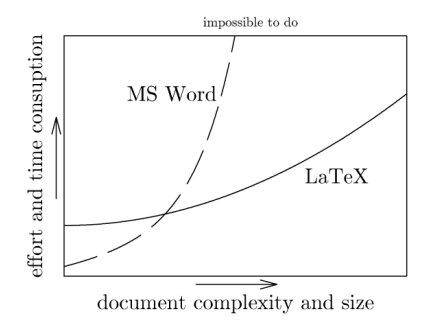
\includegraphics[ width=0.6\linewidth ]{ease-graph.png} %no te the o p ti o n a l argument to a dj u s t i t s
\caption{This graph by Marko Pinteric is spot on. }
\label{fig : vanilla}
\end{figure}		
\clearpage


\section{Basic Document Formatting}
\label{formatting}
\renewcommand{\baselinestretch}{0.5}
In STEM, brevity is highly valued. You want to put forth your arguments as crisply as possible. Of course, sometimes a rather long clarification may be in order\footnote{Footnotes are a classy way to do that. Making footnotes is fairly simple in \LaTeX\ .}, however, it is better to stick to the central theme and not disrupt the flow. In order to make your point, lists are often the cleanest option.\\
\renewcommand{\baselinestretch}{1}
\vspace{8pt}
\setlength{\parindent}{0em}\large{\textbf{ Features we demonstrate}}
\normalsize
\begin{itemize}[itemsep=-1pt]
	\item Making a title and table of contents
	\item Organising the document into sections
	\item Setting up the page layout
	\item Designing our custom header and footer
	\item Formatting text
	\item Making (nested) lists
	\begin{enumerate}[noitemsep]
		\item itemize
		\item enumerate 
		\item description
	\end{enumerate}	
	\item Footnotes
	\item Typesetting mathematics
	\item Theorem and Proof environments
	\item Hyperlinks and cross references within the document 
	\item Custom environments
	\item Algorithms and code
	\item Inserting images
	\item Drawing tables
	\item \renewcommand{\thefootnote}{\fnsymbol{footnote}}
			Citations \footnote{using Bib\TeX\, which automatically takes care of the bibliography formatting}
\end{itemize}	
In order to make your lists appear more concise, you can specify the \verb!itemsep! parameter as am optional argument to the environment. You will need the \verb!enumitem! package for that.



Descriptive lists are sometimes handy:


\begin{description}[itemsep=-5pt]
	\item [CS 207] Discrete Structures
	\item [CS 213] Data Structures and Algorithms
	\item [CS 215] Data Analysis and Interpretation
	\item [CS 251] Software Systems Lab
	\item [CS 293] Data Structures and Algorithms Lab
\end{description}	






\large{\textbf{The Page Layout}}
\normalsize

The paper size for this document is A4. The left and right margins are 1.2 inches each; the lower margin is 1.5 inches. The \verb!geometry! package is very convenient to set up and manipulate these dimensions.


\clearpage
\section{Mathematics}
\label{maths}
\renewcommand{\baselinestretch}{-1}
Make sure you have imported the \verb!amsmath!, \verb!amsthm!, \verb!amssymb!, and \verb!esint! packages, in that order. Have a look at the tutorial to understand how they work, and what theydo. In particular the \verb!amsthm! package makes defining ordered theorem-like environments very convinient.



\begin{theorem}[Markov's Inequality]
\label{markov's}
If X is a non-negative random variable and a $ > $ 0 then
\begin{equation*}
P( X \geq a) \leq \frac{E( X )}{a}
\end{equation*}

\end{theorem}

\begin{corollary}[Chebyshev's Inequality]
\label{chebyshev's}
Let X be an integrable random variable with finite expected value $\mu$ and finite variance $\sigma^2$ $\ne$ $0$. Then for any $k \in \mathbb{R},~ k > 0$,  
\begin{equation*}
P(|X - \mu| \geq k\sigma) \leq \frac{1}{k^2}
\end{equation*}

\end{corollary}
\begin{proof}
Let the random variable $Y := (X - \mu)^2$. Observe that Y is a non-negative random variable; and from the definition of variance, $E(Y) = \sigma^2$, which is positive from the premise. Hence, we can appeal to Theorem \ref{markov's}
\begin{equation*}
P(Y \geq k^2\sigma^2) \leq \frac{\sigma^2}{k^2\sigma^2} = \frac{1}{k^2}
\end{equation*}
However, $P(Y \geq k^2\sigma^2) = P(|X - \mu| \geq k\sigma)$ and we are done.
\end{proof} 
Consider a plane $z = ax + by +c$. Usually, three points on the plane are sufficient to determine the parameters  $a$, $b$, $c$; however, we're given a data set of several points: $x$ and $y$ coordinates are known perfectly, but the $z$ coordinates are corrupted by a Gaussian noise $\mathcal{N}(0,1)$. Here's how we solve for the maximum likelihood estimates of the parameters:
\begin{equation}\label{matrix}
\begin{bmatrix}
		\sum_{i}x_{i}^2	 &  \sum_{i}x_{i}{i}y_{i}   &  \sum_{i}x_{i} \\
		\sum_{i}x_{i}y_{i}	 &  \sum_{i}y_{i}^2   &  \sum_{i}y_{i}  \\
		\sum_{i}x_{i}	&   \sum_{i}y_{i}   &  \sum_{i}1   \\ 
\end{bmatrix}
\begin{bmatrix}
	\hat{a}  \\  \hat{b}  \\ \hat{c}
\end{bmatrix} = 
\begin{bmatrix}
	\sum_{i}x_{i}z_{i}  \\ \sum_{i}y_{i}z_{i}	\\ \sum_{i}z_{i}
\end{bmatrix}
\end{equation}
The above equaion (we can also refer to it as equation \ref{matrix} as we created a label) is obtained by setting the partial derivatives of the log-liklihood to 0, e.g. $\partial \mathcal{L}/\partial a = 0$ etc.




Observe that we also cross referenced Theorem \ref{markov's} in the proof of Corollary \ref{chebyshev's}. And here we just did it again. This is how we use labels in tandem with the \verb!hyperref! package.
\begin{theorem}[De Morgan's Law]
\label{morgan}
$\neg (a \lor b) \iff \neg a~\land~\neg b$ 
Alternately, in the context of sets, we have $\overline{\rm A \cup B} = \overline{\rm A} \cap \overline{\rm B}$.



\begin{remark}
This is closely related to the following rule in the first order propositional logic: $\neg(\exists x.p(x)) \iff \forall x.\neg(p(x))$
\end{remark}
\end{theorem}	



We almost always want to site sources for the claims we make, because when you publish, it's pointless to keep reinventing the wheel. For instance, the Kronecker's Theorem on simultaneous Diophantine approximations is a standard but powerful result, it makes sense to refer the reader to \cite[Chap. 7, Sec. 1.3, Prop. 7]{bourbaki1966general} for a statement and proof. This source is a book. Make sure you enter the relevant information in the appropriate fields in the BibTeX entry.


In Computer Science, most citations are journal or conference papers. A discussion on algebraic numbers is incomplete without citing the Mignotte separation bounds, given in a modestly titled conference paper \cite{mignotte1982some}. We can even cite multiple sources with a single command \cite{bell2007positivity,renegar1992computational}. These are journal articles. If possible, it's best to also specify the volume and page numbers. Your aim should be to point the reader to what you're quoting as unambiguously as possible.
\clearpage
\renewcommand{\baselinestretch}{1}
\section{Computer Science}
\label{cs}
	\subsection{Algorithms}


	We have used the \verb!algorithm2e! package.


	\begin{algorithm}
	\DontPrintSemicolon
	\KwData{Graph, source}
	\KwResult{Distances of each vertex from the source and starting edges of the shortest paths}
	create priority queue \textit{Q} of vertices of Graph //min-heap\;
	\ForEach{$vertex$ $v$ $in$ $Graph$}{
		$dist[v]\leftarrow \infty$\;
		$prev[v]\leftarrow$ UNDEFINED\;
		$add$ $v$ $to$ $Q$\;
	}
	$dist[source]\leftarrow 0$\;
		\While{$Q$ $is$ $not$ $empty$}{
			$u\leftarrow Q.extract()$\;
			\ForEach{$neighbour$ $v \in Q$  $of$ $u$}{
				$alt\leftarrow dist[u]+length(u,v)$\;
				\If{$alt<dist[v]$}{
				$dist[v]\leftarrow alt$\;
				$prev[v]\leftarrow u$\;
			}
		}
	}
	\Return{$dist[], prev[]$}\;
	\caption{Dijkstra's Algorithm}\label{shortest_distance}
	\end{algorithm}


	\subsection{Environments \& Code}

	
\subsubsection*{}
	\label{list:1}
	\begin{center}
		\textbf{\large Listing 1: [LaTeX]TeX}
		\\
		\textbf{\small The Listings Package}

	\end{center}


	\lstnewenvironment{case}
	{
	\lstset
	{
    language=[LaTeX]TeX,
    breaklines=true,
    %basicstyle=\ttfamily,
    keywordstyle=\color{blue}\textbf,
    numbers=left,
    stepnumber=1,
    showstringspaces=false,
    tabsize=1,
    commentstyle=\color{DarkGreen},
    numberstyle=\tiny\color{gray},
    stringstyle=\color{Maroon},
    showspaces=false,                
    showstringspaces=false,
	}
	} 
	{
	}
	
	%\begin{document}
	%[caption=\textbf{\large{{[LaTeX]}TeX}}\\ \textbf{\small The Listings Package},label={list:1},language={[LaTeX]TeX}]
	\raggedright
	\begin{case}
	\begin{lstlisting}
	%Your code goes here.

	%This is usually how to present code in \LaTeX, without worrying about accidentally invoking a macro. Yes, the text is displayed verbatim.
	\end{lstlisting}
	\label{trickq}
	\end{case}

	%\end{document}


	For our document, however, we noticed that na\"ive methods don’t work, and defined a custom environment with \verb!\lstnewenvironment!. This takes care of title formatting and vertical spacing too! Our environment has a counter associated with it, and takes the language and title as arguments. Other code formatting options are specified with \verb!\lstset{...}!. You might want to have a look at the tutorial!


\clearpage
\subsubsection*{}
	\label{list:2}
	\begin{center}
		\textbf{\large Listing 2: [LaTeX]TeX}
		\\
		\normalsize
		\textbf{ Algorithm Boilerplate}

	\end{center}



	\lstset
	{
    language=[LaTeX]TeX,
    breaklines=true,
    %basicstyle=\ttfamily,
    keywordstyle=\color{blue}\textbf,
    numbers=left,
    stepnumber=1,
    showstringspaces=false,
    tabsize=1,
    commentstyle=\color{DarkGreen},
    numberstyle=\tiny\color{gray},
    stringstyle=\color{Maroon},
    showspaces=false,                
    showstringspaces=false
	}
	%\begin{document}
	%[caption=\textbf{\large{{[LaTeX]}TeX}}\\Algorithm Boilerplate,label={list:2},language={[LaTeX]TeX}]
	\raggedright
	\begin{lstlisting}
	\documentclass{article}
	%...
	\usepackage[linesnumbered, ruled, vlined]{algorithm2e} 
	%...
	\begin{document}
	%...
	\begin{algorithm}[h]
	\caption{...}
	\SetAlgoLined
	\DontPrintSemicolon
	\KwData{...}
	\KwResult{...}
	Statement \ ;
	%Let magic happen here
	$1+1=2$ \ ;
	\end{algorithm}
	%...
	\end{document}
	\end{lstlisting}

	
\subsubsection*{}
	\begin{center}
		\textbf{\large Listing 3: Bash}
		\\
		\normalsize
		\textbf{ Another Language}
\normalsize
	\end{center}



	\lstset
	{
    language=Bash,
    breaklines=true,
    %basicstyle=\ttfamily,
    keywordstyle=\color{blue}\textbf,
    numbers=left,
    stepnumber=1,
    showstringspaces=false,
    tabsize=1,
    commentstyle=\color{DarkGreen},
    numberstyle=\tiny\color{gray},
    showspaces=false,                
    showstringspaces=false
	}
	%\begin{document}
	\raggedright
	\begin{lstlisting} 
	#some keywords
	for echo cat case if esac elif fi awk sed pwd while do
	sudo apt−get update sleep
	\end{lstlisting}


\subsubsection*{}
	\begin{center}
		\textbf{\large Listing 4: Python}
		\\
		\normalsize
		\textbf{ Keywords, comments, strings}

	\end{center}



	\lstset
	{
    language=Python,
    breaklines=true,
    %basicstyle=\ttfamily,
    keywordstyle=\color{blue}\textbf,
    numbers=left,
    stepnumber=1,
    showstringspaces=true,
    tabsize=1,
    commentstyle=\color{DarkGreen},
    numberstyle=\tiny\color{gray},
    stringstyle=\color{voilet},
    showspaces=false,                
	}
	%\begin{document}
	\raggedright
	\begin{lstlisting} 
	from numpy import *
	#insanely powerful library
	print("Hello Everyone!")
	\end{lstlisting}



	The advantage of defining ordered environments like this is that you can refer to this pretty easily if
	you’ve left a label properly. If you want to shift them around, the counter and the cross references
	will do the adjustment automatically. Of the above, Listing \hyperlink{page.4}{1} is a fiendish trick question, and
	Listing \hyperlink{page.5}{2} is rather benevolent.
\clearpage
\renewcommand{\baselinestretch}{1}
\section{Utilities}
\label{utils}
	\subsection{Images}

	\renewcommand{\baselinestretch}{0.5}
	You'll sometimes find the need to include images in your report. Ideally, the image should enhance the document. But yeah, you're probably going to use this technique for a rather dirty life hack. If a prop insists on a \LaTeX\ report, you're just going to dump a photo of your exquisite handwriting to save time, aren't you? \textit{Exploit this loophole at your own risk. The original author of this assignment can neither confirm nor deny his endorsement of the jugaad.}
	%\renewcommand{\baselinestretch}{1}
	\begin{figure}[h]
	\centering
	\begin{floatrow}
	\ffigbox{\caption{Aristotle: The first formal logician}}{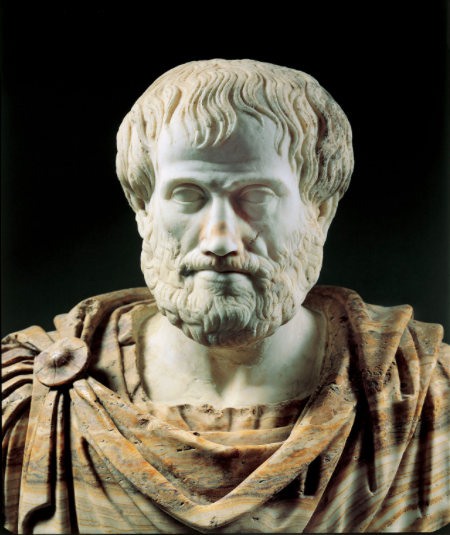
\includegraphics[height=7cm]{aristotle.png}} \ffigbox{\caption{Saul Kripke: we've come a long way since then}}{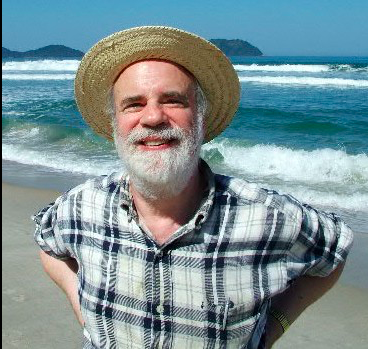
\includegraphics[height=7cm]{kripke.png}}
	\end{floatrow}
	\end{figure}\\
	\href{https://www.britannica.com/biography/Aristotle}{Aristotle image source}\\
	\href{https://commons.wikimedia.org/w/index.php?curid=5763037}{Saul Kripke image source}\\
	Make sure you follow these links, so you know where the hyperlinks lead to when you typeset it yourself.
	\subsection{Tables}
	\renewcommand{\baselinestretch}{1}
	%\begin{adjustwidth}{-2cm}{}
	\begin{table}[h]
		
		\begin{flushleft}
		\centering
		\begin{tabular}{@{}c|l@{}}
		\hline
		\mycell{\textbf{Complexity}}{\textbf{Examples}}
		\hline
		\mycell{$\mathcal{O}(1)$}{Computing $(-1)^n$}
		\hline
		\mycell{\myrow{$\mathcal{O}(log(n))$}}{Binary Search}
		%\mycell{a}{}
		\mycell{}{Insertion \& Removal from a min-heap}
		\hline
		\mycell{\myrow{$\mathcal{O}(nlog(n))$}}{Merge Sort}
		\mycell{}{Fast Fourier Transform}
		\hline
		\mycell{\myrow{$\mathcal{O}(n^2)$}}{Bubble Sort}
		\mycell{}{First attempt at a problem which has a linear time solution}
		\hline
		\mycell{$2^{\mathcal{O}(log(n))}$}{AKS Primality Test}
		\hline
		\multicolumn{2}{c}{You might want to define a macro to write this notation conveniently} \\
		\hline
		\end{tabular}
		\end{flushleft}
		\caption{Some common time complexities}
	\end{table}	
	\renewcommand{\baselinestretch}{0.5}
	This table uses \verb!multirow! as well as \verb!multicolumn!. Replicate it as well as you can. 
	\clearpage
	\renewcommand{\baselinestretch}{1}
	We have used the fairly popular \verb!plainurl! style.
	\bibliographystyle{plainurl}
	\bibliography{my_starter_pack}


%What is a quiet comment?
\end{document}